\documentclass[10pt]{beamer}

\usetheme[progressbar=frametitle]{metropolis}
\usepackage{appendixnumberbeamer}

\usepackage{booktabs}
\usepackage[scale=2]{ccicons}

\usepackage{pgfplots}
\usepgfplotslibrary{dateplot}

\usepackage{xspace}
\newcommand{\themename}{\textbf{\textsc{metropolis}}\xspace}

\title{IDP}
\subtitle{Fixed-Point Matrix Multiplication}
% \date{\today}
\date{}
\author{Pamula Bhargav Ram\\EE16BTECH11024\\Rallabandi Rishideep Reddy\\EE16BTECH11031}
\institute{Problem statement and Implementation Strategy}
% \titlegraphic{\hfill\includegraphics[height=1.5cm]{logo.pdf}}

\begin{document}

\maketitle

\begin{frame}{Table of contents}
  \setbeamertemplate{section in toc}[sections numbered]
  \tableofcontents[hideallsubsections]
\end{frame}

\section{Introduction}

\begin{frame}[fragile]{Fixed Point Matrix Multiplication}

  The main idea of fixed point arithematic is to interpret bit words as integers coupled with a scale factor: \( \displaystyle \frac{z}{2^n} \)
  \begin{figure}
    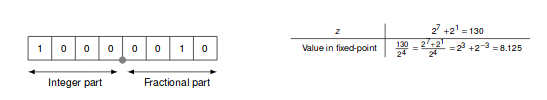
\includegraphics[scale=0.6]{Fixed.png}
  \end{figure}
  Multiplication: The product of a \(Q_{a,b}\) variable by a \(Q_{c,d}\) yields a \(Q_{a+b,c+d}\) variable.
  \begin{figure}
    {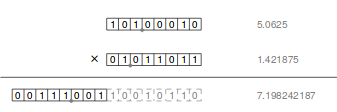
\includegraphics[scale=0.5]{MULTI.png}}
  \end{figure}
\end{frame}
\begin{frame}{Fixed Point Matrix Multiplication}
  \begin{figure}
    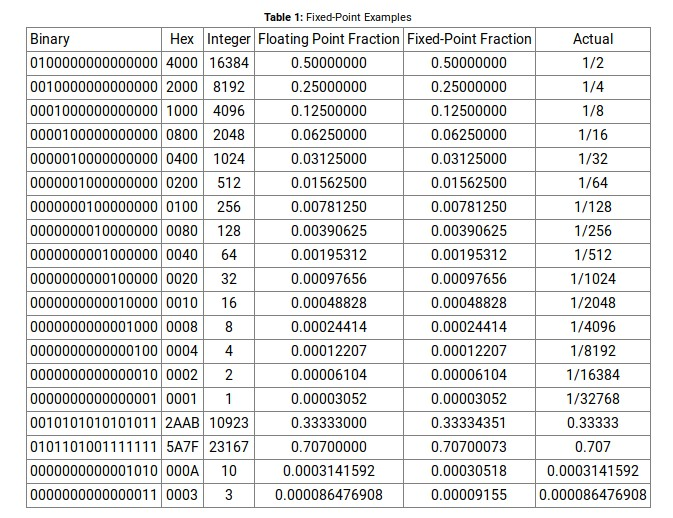
\includegraphics[scale=0.45]{Fixed_point.jpg}
  \end{figure}
\end{frame}
\begin{frame}[fragile]{Fixed Point Matrix Multiplication}
\begin{itemize}
    \item It is similar to a normal matrix multiplication, whereas here we use fixed point multiplication between the numbers.
    \item
    The input is stored in the BRAM memory block and after the computation output is also stored in BRAM memory block
\end{itemize}
    
\end{frame}


\section{Problem Statement}

\begin{frame}{Problem Statement}
	\begin{itemize}
		\item input matrices will be taken from keypad.
		\item fixed point numbers must be used to multiply and generate a matrix in Ico board (result of multiplication of two matrices).
		\item the output will be displayed via Arduino.
	\end{itemize}
	
\end{frame}

\section{Implementation Strategy}

\begin{frame}[fragile]{Implementation Strategy}
	\begin{itemize}
		\item mode of input is keypad which is connected to Arduino.
		\item Arduino converts floating point input to fixed point output. 
		\item Ico board receives input from Arduino where matrix multiplication is programmed.
		\item Ico board sends the output after the multiplication process to Arduino.
		\item The output matrix can be displayed in Arduino-python interface after floating point conversion.
	\end{itemize}
	The Project will be implemented for (\(3\times3\)) matrix. And 8-bit fixed-point numbers will be used.
\end{frame}
\section{Updates till now}
\begin{frame}{Updates}
    \begin{itemize}
        \item implemented multipliction of two $(4\times4)$ matrices in verilog.
        \item The input for the matrices are signed 8-bit each and output is signed 11-bit.
        \item The algorithm for Arduino to convert decimal inputs to binary output is completed. Inputs are taken from Serial monitor using Serial.read and then converted to binary and fractional binary.
    \end{itemize}
    
\end{frame}
{\setbeamercolor{palette primary}{fg=white, bg=blue!20}
\begin{frame}[standout]
  \Huge{THANK YOU}
\end{frame}
}


\end{document}
